\subsection{Data}


We construct a collection of relatively high-quality video clips with text descriptions through video filters and recaption models. % based on CogVLM2~\cite{wang2023cogvlm}. 
After filtering, approximately 35M single-shot clips remain, with each clip averaging about 6 seconds. 



\paragraph{Video Filtering.}
Video generation models need to learn the dynamic information of the world, but unfiltered video data is of highly noisy distribution, primarily due to two reasons: 
First, videos are human-created, and artificial editing may distort the authentic dynamic information; 
Second, the quality of videos can significantly drop due to issues during filming, such as camera shakes and substandard equipment.

In addition to the intrinsic quality of the videos, we also consider how well the video data supports model training. 
Videos with minimal dynamic information or lacking connectivity in dynamic aspects are considered detrimental. 
Consequently, we have developed a set of negative labels, which include:

\begin{itemize}
    \item \textbf{Editing}: Videos that have undergone obvious artificial processing, such as re-editing and special effects, causing degradation of the visual integrity.
    \item \textbf{Lack of Motion Connectivity}: Video segments with image transitions lacking motion connectivity, commonly seen in videos artificially spliced or edited from images.
    \item \textbf{Low Quality}: Poorly shot videos with unclear visuals or excessive camera shake.
    \item \textbf{Lecture Type}: Videos focusing primarily on a person continuously talking with minimal effective motion, such as educational content, lectures, and live-streamed discussions.
    \item \textbf{Text Dominated}: Videos containing a substantial amount of visible text or primarily focusing on textual content.
    \item \textbf{Noisy Screenshots}: Noisy videos recorded from phone or computer screens.
\end{itemize}

We sample 20,000 video data samples and label the presence of negative tags in each of them. 
By using these annotations, we train several filters based on video-llama~\citep{zhang2023video}  to screen out low-quality video data. 


In addition, we calculate the optical flow scores and image aesthetic scores of all training videos and dynamically adjust the threshold ranges during training  to ensure the fluency and aesthetic quality of the generated videos. 




\paragraph{Video Caption.} 
Typically, most video data does not come with corresponding descriptive text, so it is necessary to convert the video data into textual descriptions to provide the essential training data for text-to-video models. 
Currently, there are some video caption datasets available, such as Panda70M~\citep{chen2024panda}, COCO Caption~\citep{lin2014microsoft}, and WebVid~\cite{bain2021frozen}. 
However, the captions in these datasets are usually very short and fail to describe the video's content comprehensively. 




\begin{figure}[h]
\begin{center}
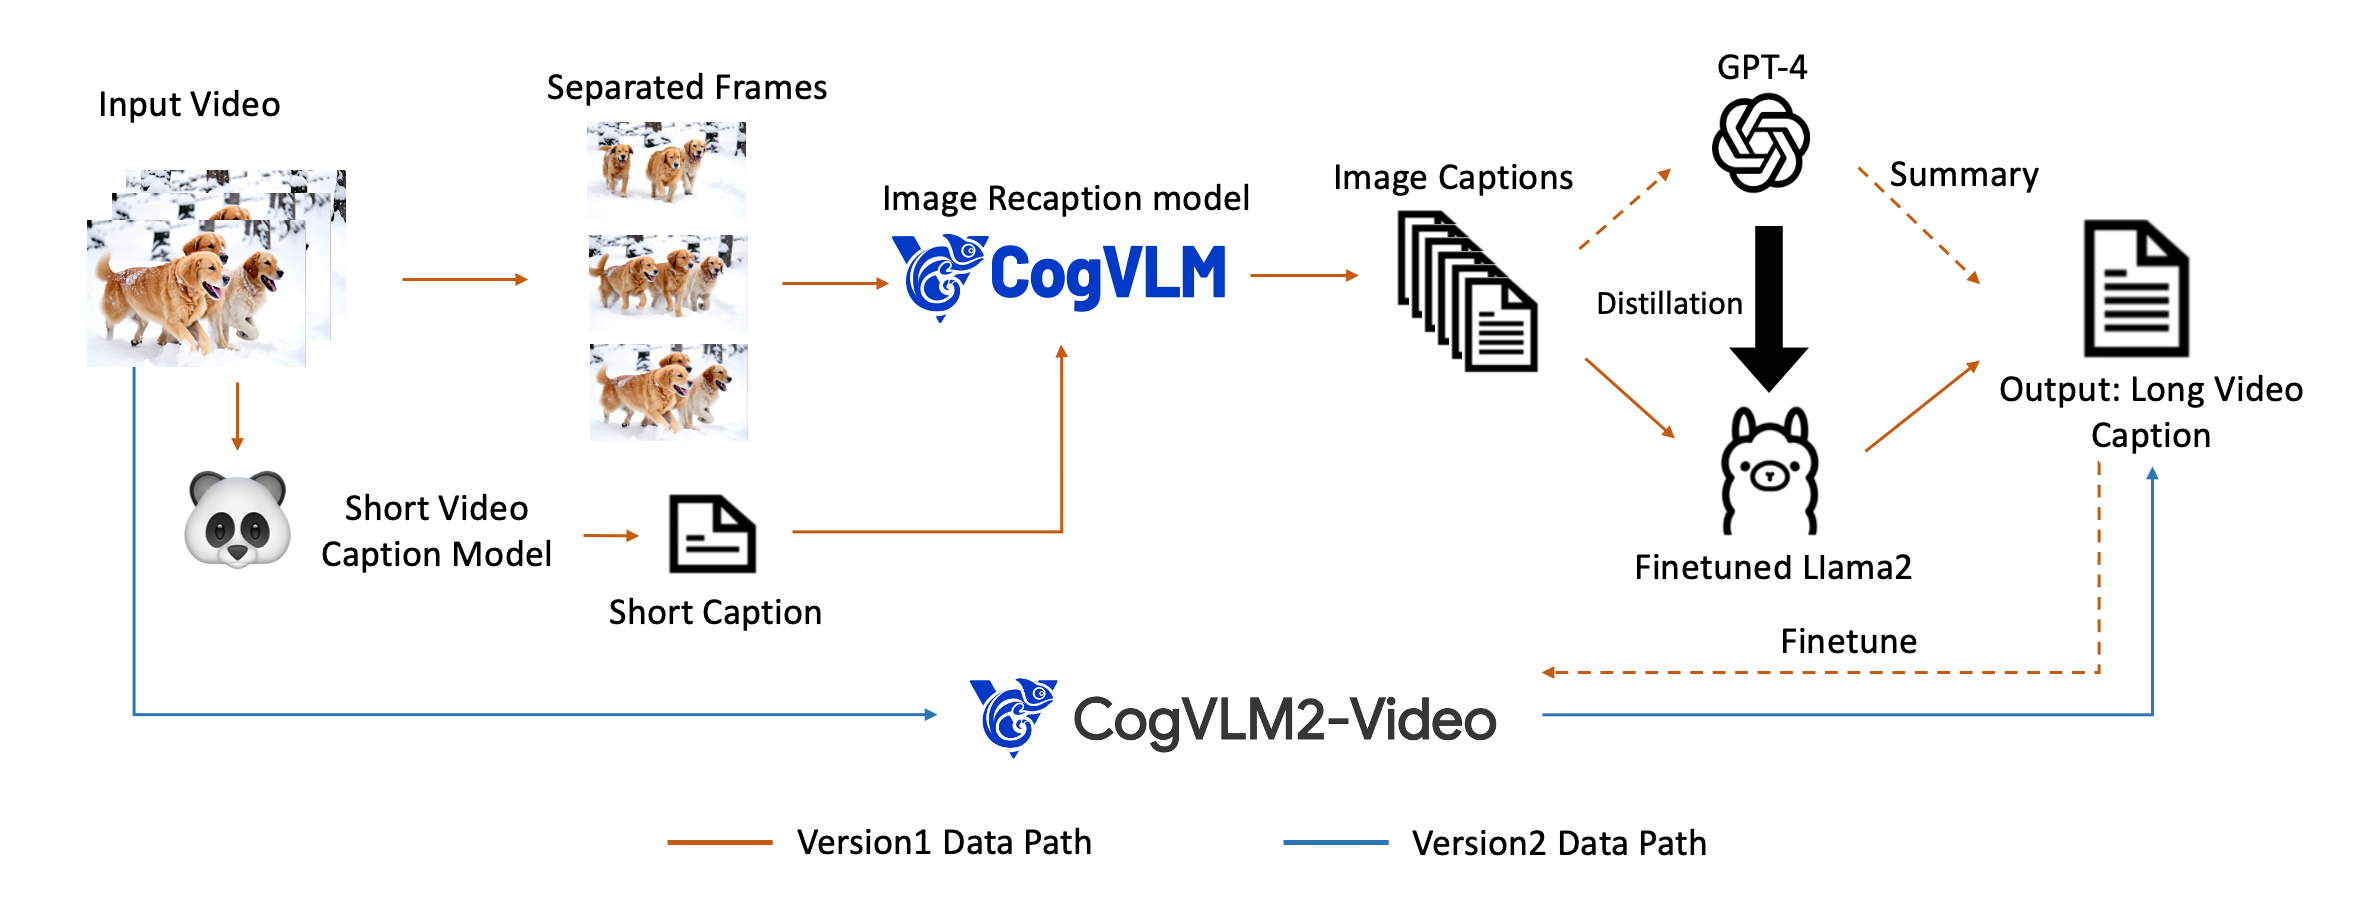
\includegraphics[width=\linewidth]{images/pipeline.jpg}
\end{center}
\caption{The pipeline for dense video caption data generation. In this pipeline, we generate short video captions with the Panda70M model, extract frames to create dense image captions, and use GPT-4 to summarize these into final video captions. To accelerate this process, we fine-tuned a Llama 2 model with the GPT-4 summaries.}
\label{fig:video_caption_gen}
\end{figure}

%\paragraph{.} 
To generate high-quality video caption data, we establish a \textit{Dense Video Caption Data Generation} 
%complex data generation 
pipeline, as detailed in Figure~\ref{fig:video_caption_gen}.  
The idea is to generate video captions from image captions. %

First, we use the Panda70M video captioning model~\citep{chen2024panda} to generate short captions for the videos. 
Then, we employ the image recaptioning model CogVLM~\citep{wang2023cogvlm} used in Stable~Diffusion~3~\citep{esser2024scaling} and CogView3~\citep{zheng2024cogview3} to create dense image captions for each of the frames within a video.  
Subsequently, we use GPT-4 to summarize all the image captions to produce the final video caption. 
To accelerate the generation from image captions to video captions, we fine-tune a Llama2 model~\citep{touvron2023llama} using the summary data generated by GPT-4~\citep{GPT4}, enabling large-scale video caption data generation. Additional details regarding the video caption data generation process can be found in Appendix~\ref{ap:video_caption_gen}.


%We thus propose to build a pipeline to generate video captions from image captions and then fine-tune an end-to-end video captioning model to obtain more dense video captions. 
%Our final video captioning model can generate more detailed descriptions of videos, further enhancing the quality of video generation \citep{betker2023improving}.
 
The pipeline above generates the caption data that is used to trained the \model model introduced in this report. 
To further accelerate video recaptioning, we also fine-tune an end-to-end video understanding model CogVLM2-Caption, based on the CogVLM2-Video\footnote{The CogVLM2-Video model weight is openly available at \url{https://github.com/THUDM/CogVLM2}.} and Llama3~\citep{llama3modelcard}, by using the dense caption data generated from the aforementioned pipeline. 
The video caption data generated by CogVLM2-Caption is used to train the next generation of \model. 
%This dense video captions. % as described above through the pipeline method. 
Examples of video captions generated by this end-to-end CogVLM2-Caption model are shown in Appendix~\ref{ap:video_caption_example}. 
In Appendix~\ref{ap:v2v}, we also present some examples of video generation where a video is first input into CogVLM2-Caption to generate captions, which are then used as input for \model to generate new videos, effectively achieving video-to-video generation.



